\section{Data Collection}

We have collected data from FDIC website with a list of failed banks since Oct
2000, which contains acquiring institutions, and another list of failed banks
since the establishment of FDIC.

We joined the two tables based on their CERT number, which is a primary key of
the tables. We filtered out any items that has N/A in the estimated loss
column, which are all in 2017. Now we have data from Oct 2000 to Dec 2016.

We also want to get the geographic coordinates (longitutde and latitude) of
the headquarters of the failed banks. We used a site called www.latlong.net.
The site has a input box where one can enter the name of a location and a
button ``find'', which loads the latitude and longitude into the other two
input boxes when clicked. This website is awesome except that the api are
hidden in a complex and lengthy JavaScript. Instead of trying to decipher the
JavaScript code, we wrote a script to emulate input and click to fetch the
coordinates for a list of locations. The script is in data/latlong.net.js,
where the first part is used to load jQuery and has to be run first
separately. After a few seconds, we can paste the remaining part of the script
into the console in Chrome. Then we set the city\_names global variable to a
list of locations we want to get coordinates for and invoke start\_first().
After a while, the results global variable is populated with a list of triple
of location name, latitude and longitude.

A note to the script: there has to be a wait after both input to the location
name box and clicking the find button. I don't know if this is due to the lag
of my system or network issue or google map needs more time to load or their
bugs. Now I set both waits at 5 seconds. On my own laptop, this allows me to
fetch more than 300 locations in a row without any error. In case an error
occurs, an alert dialog (which is part of the website's design, not mine),
will pop up saying invalid location. When this happens, the current location
in the input box has better to be recorded so that we can come back to do it
again (manually of course). The remainder of the script will typically run as
usual. From my personal experience, when the number of location gets near 400,
the error starts to pop up every 1 or 2 locations. I had to manually correct
about 40 locations.

We then joined the coordinates with the data. Some of the data are in Puerto
Rico, which cannot be correctly displayed by d3.geoAlbersUsa(). We simply
filtered out those records.

\newpage

\section{Screenshot before milestone (Nov 10, 2017)}

\begin{figure}[!h]
    \centering
    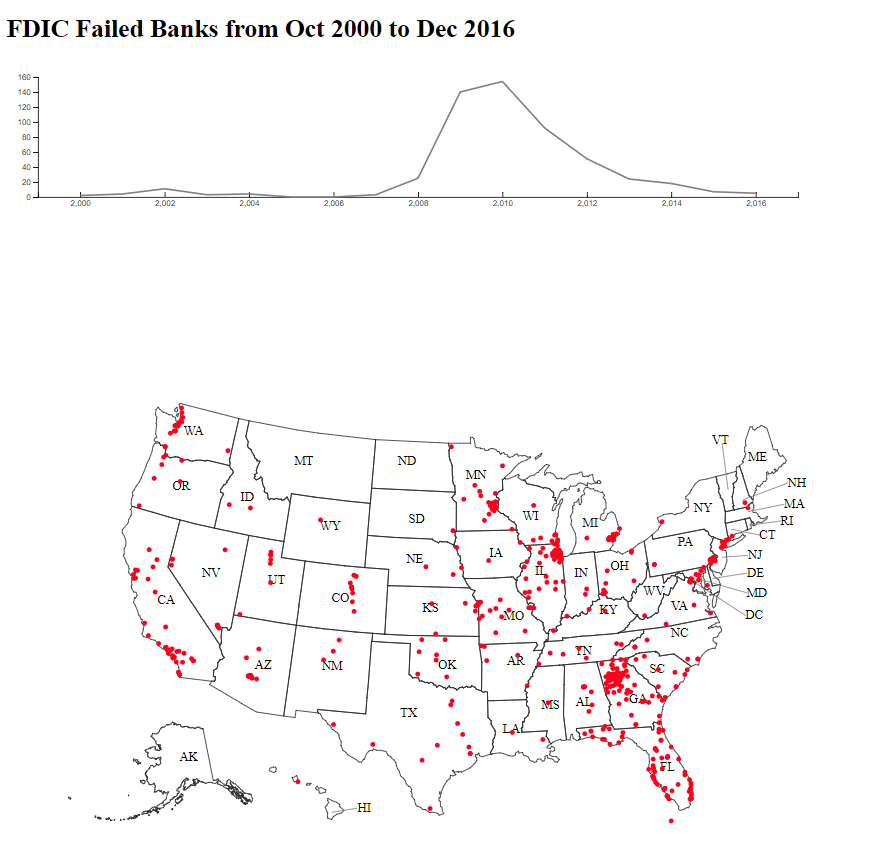
\includegraphics[width=\textwidth]{fig/Nov10}
    \caption{A screenshot for the milestone as of November 10}
    \label{fig:milestone}
\end{figure}

Now, this is what we have (see Figure \ref{fig:milestone}) as of the milestone
(Nov 10, 2017). We have the line chart and the map set up with the bar chart
yet to complete. 

The line chart still doesn't have a drop-down list to select
the y-axis, which is currently the number of failed banks in a year. We plan
to add a dots to the line chart so that a user can easily select one or some
of the years. We also plan to add tooltips to each dot so that the exact
number is easy to read, as some of them are quite small compared to those of
2008-2010.

The map hasn't been linked to the line chart and only plots the full dataset.
As shown in the figure, some areas has dense population of failed banks,
making it hard to use tooltip to show the details. And some of the banks are
in the same city (e.g., surprisingly 19 in Chicago, IL, 10 in Atlanta, GA,
while New York City only has 2), which also makes tooltip infeasible. Instead
of tooltips, we plan to use 2D brush to select a range of banks. And we'll
show a list of those banks. The user can click on one of them to expand the
detailed information about it on a separate box.

Hopefully, our work will have a functioning line chart and map by the next
week.
